\documentclass[11pt]{beamer}
% \usetheme{Boadilla}
  \usetheme{default}


% math mode only
\newcommand {\Lmax} {L_{\mbox{\small max}}}
\newcommand {\Vmax} {V_{\mbox{\small max}}}



\title{interferometric interpolation}
\author{H.~E.~Motteler}
\institute{
  UMBC Atmospheric Spectroscopy Lab \\
  Joint Center for Earth Systems Technology \\
}
\date{\today}
\begin{document}

%----------- slide --------------------------------------------------%
\begin{frame}[plain]
\titlepage
\end{frame}
%----------- slide --------------------------------------------------%
\begin{frame}
\frametitle{basic equations}

The Nyquist equations for Fourier transform interferometry are

\[ V = N \/dv = 1/ 2\/dx \]
\[ L = N \/dx = 1/ 2\/dv \]

where

\begin{itemize}
  \item $L$ is maximum OPD
  \item $V$ is maximum frequency
  \item $dx$ is the distance step
  \item $dv$ is the frequency step
  \item the transform size is $2N$
\end{itemize}

\end{frame}
%----------- slide --------------------------------------------------%
\begin{frame}
\frametitle{example}

\begin{center}
  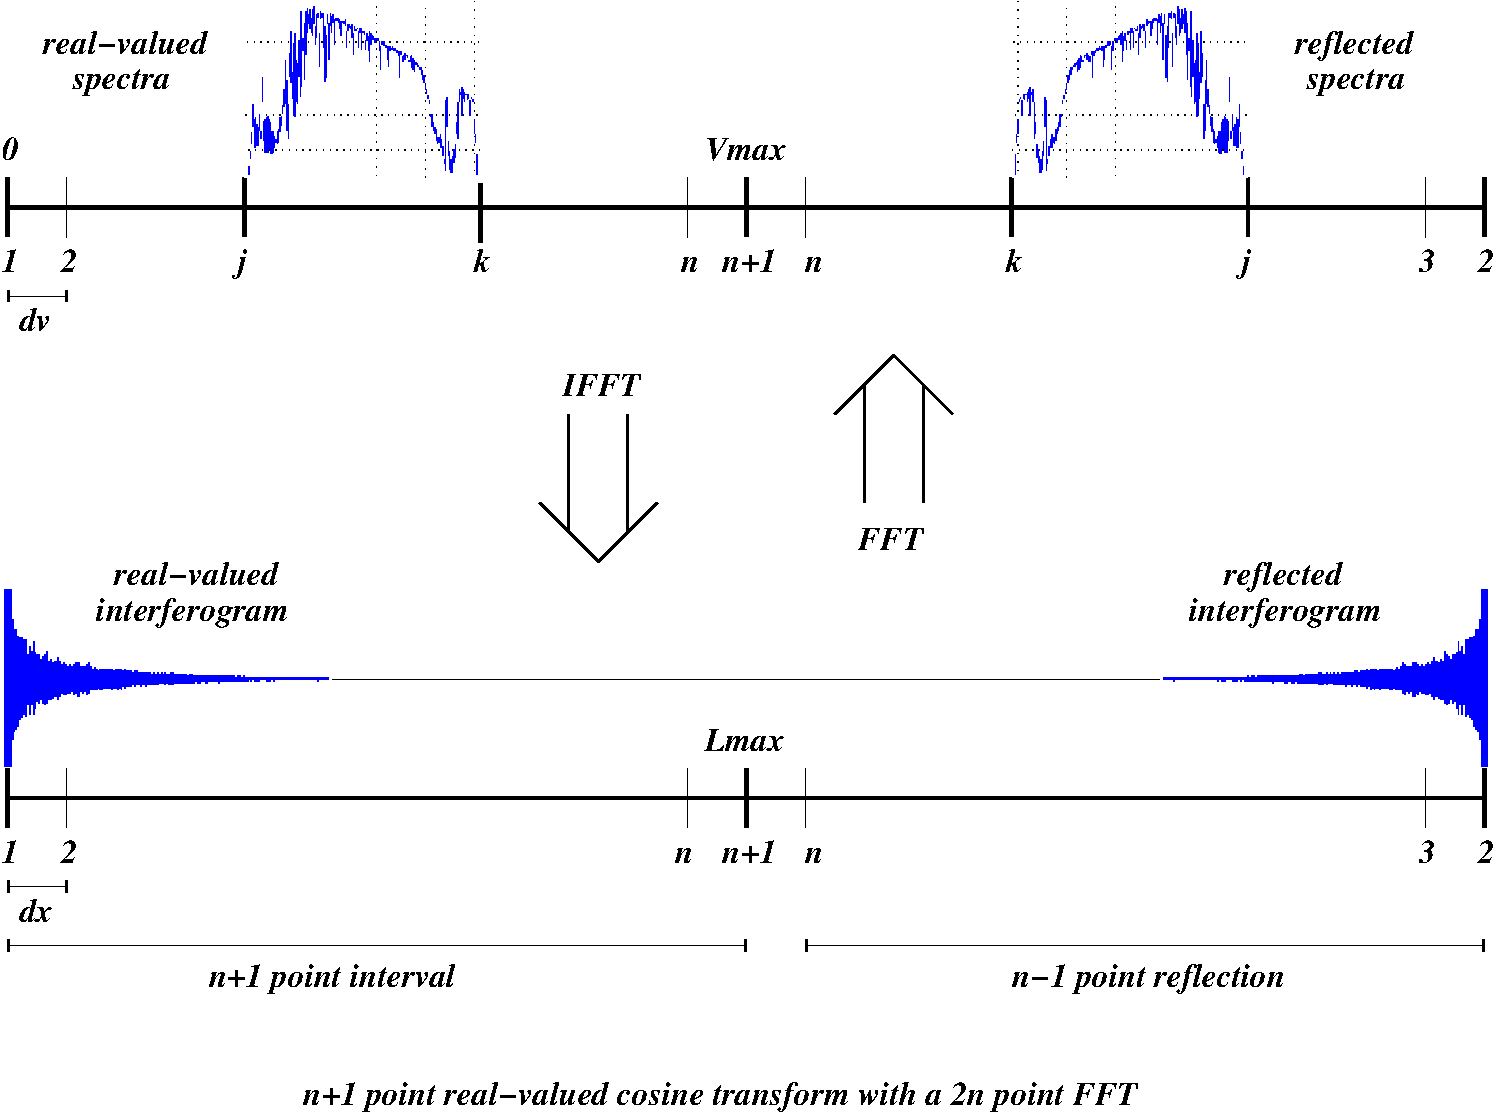
\includegraphics[scale=0.4]{figures/cos_tfrm.pdf}
\end{center}

\end{frame}
%----------- slide --------------------------------------------------%
\begin{frame}
\frametitle{discussion}

\begin{itemize}
  \item the previous slide shows the special case of a symmetrical
    real-valued interferogram being transformed to symmetrical
    real-valued spectra.  Note that the transform is invertible.
  \item the $2n$ point real-valued FFT is equivalent to an $n+1$
    point cosine transform.
  \item applications of the $n+1$ point representation include
    \begin{itemize}
       \item calculating expected observed radiances
       \item applying apodization and response functions
       \item interpolation between instrument grids
    \end{itemize}
  \item for a typical interpolation application we start with two
    frequency steps, $dv_1$ and $dv_2$, and want to move between
    them
\end{itemize}

\end{frame}
%----------- slide --------------------------------------------------%
\begin{frame}
\frametitle{interpolation}

\begin{center}
  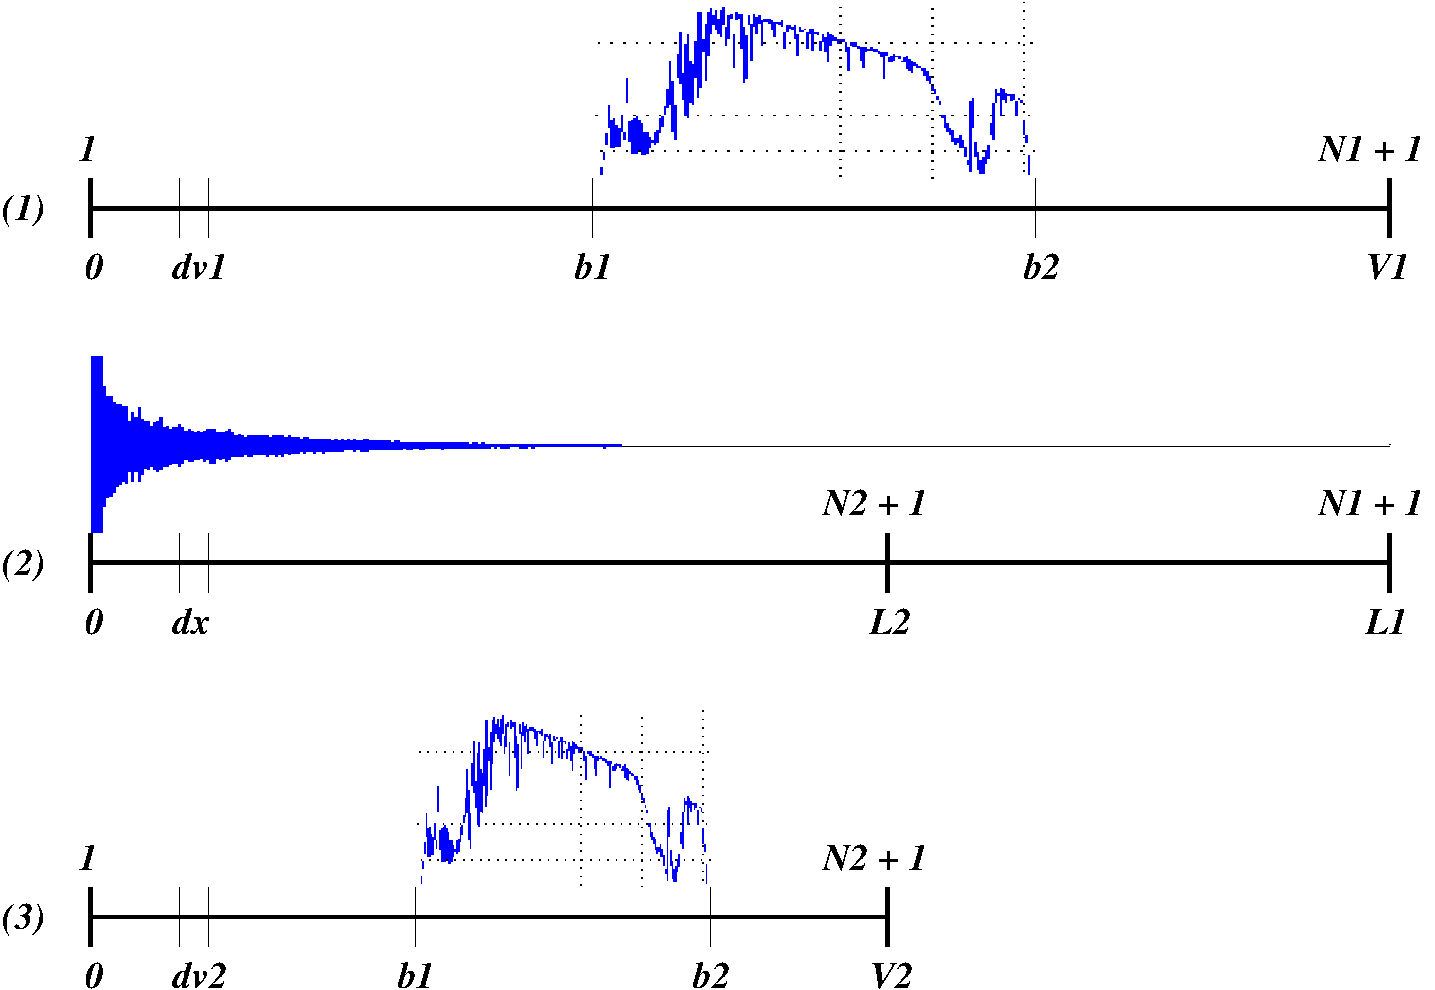
\includegraphics[scale=0.4]{figures/interp_tfrm.pdf}
\end{center}

\end{frame}
%----------- slide --------------------------------------------------%
\begin{frame}
\frametitle{basic equations}

The Nyquist equations for (1) and (2) are

\[ V_1 = N_1 \/dv_1 = 1/ 2\/dx \]
\[ L_1 = N_1 \/dx   = 1/ 2\/dv_1 \]

and for (2) and (3) are

\[ V_2 = N_2 \/dv_2 = 1/ 2\/dx \]
\[ L_2 = N_2 \/dx   = 1/ 2\/dv_2 \]

If we are given $dv_1$ and $dv_2$ then we need $dx$, $N_1$, or $N_2$
to fill out the values above.  $N_1$ and $N_2$ must be integers.

\end{frame}
%----------- slide --------------------------------------------------%
\begin{frame}
\frametitle{constraints}

Note that $dx$ is the same for both pairs of equations, so $V_1 =
V_2$.  Then $N_1\/dv_1 = N_2\/dv_2$, and we have

\[ N_2 / N_1 = dv_1 / dv_2, \]

a constraint on the transform sizes that can only be satisfied if
$dv_1 / dv_2$ is rational.  In addition, the transforms must include
the band of interest, so we require 

\[ V_1 = N_1\/dv_1 \ge b_2 \]

Suppose $dv_1 / dv_2$ is rational.  Let $m_1$ and $m_2$ be the smallest
integers such that $m_1/m_2 = dv_1 / dv_2$. \\

\end{frame}
%----------- slide --------------------------------------------------%
\begin{frame}
\frametitle{constraints}

Let $k$ be the smallest integer such that $m_2 \cdot 2^k \cdot dv_1
\ge b_2$, and let $N_1 = m_2 \cdot 2^k$ and $N_2 = m_1 \cdot 2^k$. \\
\bigskip
Then the constraints above are satisfied, and in addition if $m_1$
and $m_2$ are not too large then $N_1$ and $N_2$ will have mostly
small prime factors, making the FFT calculation more efficient. \\
\bigskip
If $dv_1 / dv_2$ is not rational or $m_1$ or $m_2$ are very large we
may want to proceed differently, for example by finding a value for
$dv_1$ close to the desired $dv$ but with a more tractible rational
representation.  In that case we might want to do a conventional
interpolation from $dv$ to $dv_1$ as a preliminary step.

\end{frame}
%----------- slide --------------------------------------------------%
\end{document}

